
%% bare_jrnl.tex
%% V1.3
%% 2007/01/11
%% by Michael Shell
%% see http://www.michaelshell.org/
%% for current contact information.
%%
%% This is a skeleton file demonstrating the use of IEEEtran.cls
%% (requires IEEEtran.cls version 1.7 or later) with an IEEE journal paper.
%%
%% Support sites:
%% http://www.michaelshell.org/tex/ieeetran/
%% http://www.ctan.org/tex-archive/macros/latex/contrib/IEEEtran/
%% and
%% http://www.ieee.org/



% *** Authors should verify (and, if needed, correct) their LaTeX system  ***
% *** with the testflow diagnostic prior to trusting their LaTeX platform ***
% *** with production work. IEEE's font choices can trigger bugs that do  ***
% *** not appear when using other class files.                            ***
% The testflow support page is at:
% http://www.michaelshell.org/tex/testflow/


%%*************************************************************************
%% Legal Notice:
%% This code is offered as-is without any warranty either expressed or
%% implied; without even the implied warranty of MERCHANTABILITY or
%% FITNESS FOR A PARTICULAR PURPOSE! 
%% User assumes all risk.
%% In no event shall IEEE or any contributor to this code be liable for
%% any damages or losses, including, but not limited to, incidental,
%% consequential, or any other damages, resulting from the use or misuse
%% of any information contained here.
%%
%% All comments are the opinions of their respective authors and are not
%% necessarily endorsed by the IEEE.
%%
%% This work is distributed under the LaTeX Project Public License (LPPL)
%% ( http://www.latex-project.org/ ) version 1.3, and may be freely used,
%% distributed and modified. A copy of the LPPL, version 1.3, is included
%% in the base LaTeX documentation of all distributions of LaTeX released
%% 2003/12/01 or later.
%% Retain all contribution notices and credits.
%% ** Modified files should be clearly indicated as such, including  **
%% ** renaming them and changing author support contact information. **
%%
%% File list of work: IEEEtran.cls, IEEEtran_HOWTO.pdf, bare_adv.tex,
%%                    bare_conf.tex, bare_jrnl.tex, bare_jrnl_compsoc.tex
%%*************************************************************************

% Note that the a4paper option is mainly intended so that authors in
% countries using A4 can easily print to A4 and see how their papers will
% look in print - the typesetting of the document will not typically be
% affected with changes in paper size (but the bottom and side margins will).
% Use the testflow package mentioned above to verify correct handling of
% both paper sizes by the user's LaTeX system.
%
% Also note that the "draftcls" or "draftclsnofoot", not "draft", option
% should be used if it is desired that the figures are to be displayed in
% draft mode.
%
\documentclass[journal]{IEEEtran}
%
% If IEEEtran.cls has not been installed into the LaTeX system files,
% manually specify the path to it like:
% \documentclass[journal]{../sty/IEEEtran}





% Some very useful LaTeX packages include:
% (uncomment the ones you want to load)


% *** MISC UTILITY PACKAGES ***
%
%\usepackage{ifpdf}
% Heiko Oberdiek's ifpdf.sty is very useful if you need conditional
% compilation based on whether the output is pdf or dvi.
% usage:
% \ifpdf
%   % pdf code
% \else
%   % dvi code
% \fi
% The latest version of ifpdf.sty can be obtained from:
% http://www.ctan.org/tex-archive/macros/latex/contrib/oberdiek/
% Also, note that IEEEtran.cls V1.7 and later provides a builtin
% \ifCLASSINFOpdf conditional that works the same way.
% When switching from latex to pdflatex and vice-versa, the compiler may
% have to be run twice to clear warning/error messages.






% *** CITATION PACKAGES ***
%
%\usepackage{cite}
% cite.sty was written by Donald Arseneau
% V1.6 and later of IEEEtran pre-defines the format of the cite.sty package
% \cite{} output to follow that of IEEE. Loading the cite package will
% result in citation numbers being automatically sorted and properly
% "compressed/ranged". e.g., [1], [9], [2], [7], [5], [6] without using
% cite.sty will become [1], [2], [5]--[7], [9] using cite.sty. cite.sty's
% \cite will automatically add leading space, if needed. Use cite.sty's
% noadjust option (cite.sty V3.8 and later) if you want to turn this off.
% cite.sty is already installed on most LaTeX systems. Be sure and use
% version 4.0 (2003-05-27) and later if using hyperref.sty. cite.sty does
% not currently provide for hyperlinked citations.
% The latest version can be obtained at:
% http://www.ctan.org/tex-archive/macros/latex/contrib/cite/
% The documentation is contained in the cite.sty file itself.



  \usepackage{hyperref}


% *** GRAPHICS RELATED PACKAGES ***
%
%\ifCLASSINFOpdf
  \usepackage[pdftex]{graphicx}
  % declare the path(s) where your graphic files are
  \graphicspath{{Images/}}
  % and their extensions so you won't have to specify these with
  % every instance of \includegraphics
  \DeclareGraphicsExtensions{.jpg,.png}
%\else
  % or other class option (dvipsone, dvipdf, if not using dvips). graphicx
  % will default to the driver specified in the system graphics.cfg if no
  % driver is specified.
  % \usepackage[dvips]{graphicx}
  % declare the path(s) where your graphic files are
  % \graphicspath{{../eps/}}
  % and their extensions so you won't have to specify these with
  % every instance of \includegraphics
  % \DeclareGraphicsExtensions{.eps}
%\fi
% graphicx was written by David Carlisle and Sebastian Rahtz. It is
% required if you want graphics, photos, etc. graphicx.sty is already
% installed on most LaTeX systems. The latest version and documentation can
% be obtained at: 
% http://www.ctan.org/tex-archive/macros/latex/required/graphics/
% Another good source of documentation is "Using Imported Graphics in
% LaTeX2e" by Keith Reckdahl which can be found as epslatex.ps or
% epslatex.pdf at: http://www.ctan.org/tex-archive/info/
%
% latex, and pdflatex in dvi mode, support graphics in encapsulated
% postscript (.eps) format. pdflatex in pdf mode supports graphics
% in .pdf, .jpeg, .png and .mps (metapost) formats. Users should ensure
% that all non-photo figures use a vector format (.eps, .pdf, .mps) and
% not a bitmapped formats (.jpeg, .png). IEEE frowns on bitmapped formats
% which can result in "jaggedy"/blurry rendering of lines and letters as
% well as large increases in file sizes.
%
% You can find documentation about the pdfTeX application at:
% http://www.tug.org/applications/pdftex





% *** MATH PACKAGES ***
%
\usepackage[cmex10]{amsmath}
% A popular package from the American Mathematical Society that provides
% many useful and powerful commands for dealing with mathematics. If using
% it, be sure to load this package with the cmex10 option to ensure that
% only type 1 fonts will utilized at all point sizes. Without this option,
% it is possible that some math symbols, particularly those within
% footnotes, will be rendered in bitmap form which will result in a
% document that can not be IEEE Xplore compliant!
%
% Also, note that the amsmath package sets \interdisplaylinepenalty to 10000
% thus preventing page breaks from occurring within multiline equations. Use:
%\interdisplaylinepenalty=2500
% after loading amsmath to restore such page breaks as IEEEtran.cls normally
% does. amsmath.sty is already installed on most LaTeX systems. The latest
% version and documentation can be obtained at:
% http://www.ctan.org/tex-archive/macros/latex/required/amslatex/math/





% *** SPECIALIZED LIST PACKAGES ***
%
%\usepackage{algorithmic}
% algorithmic.sty was written by Peter Williams and Rogerio Brito.
% This package provides an algorithmic environment fo describing algorithms.
% You can use the algorithmic environment in-text or within a figure
% environment to provide for a floating algorithm. Do NOT use the algorithm
% floating environment provided by algorithm.sty (by the same authors) or
% algorithm2e.sty (by Christophe Fiorio) as IEEE does not use dedicated
% algorithm float types and packages that provide these will not provide
% correct IEEE style captions. The latest version and documentation of
% algorithmic.sty can be obtained at:
% http://www.ctan.org/tex-archive/macros/latex/contrib/algorithms/
% There is also a support site at:
% http://algorithms.berlios.de/index.html
% Also of interest may be the (relatively newer and more customizable)
% algorithmicx.sty package by Szasz Janos:
% http://www.ctan.org/tex-archive/macros/latex/contrib/algorithmicx/




% *** ALIGNMENT PACKAGES ***
%
%\usepackage{array}
% Frank Mittelbach's and David Carlisle's array.sty patches and improves
% the standard LaTeX2e array and tabular environments to provide better
% appearance and additional user controls. As the default LaTeX2e table
% generation code is lacking to the point of almost being broken with
% respect to the quality of the end results, all users are strongly
% advised to use an enhanced (at the very least that provided by array.sty)
% set of table tools. array.sty is already installed on most systems. The
% latest version and documentation can be obtained at:
% http://www.ctan.org/tex-archive/macros/latex/required/tools/


%\usepackage{mdwmath}
%\usepackage{mdwtab}
% Also highly recommended is Mark Wooding's extremely powerful MDW tools,
% especially mdwmath.sty and mdwtab.sty which are used to format equations
% and tables, respectively. The MDWtools set is already installed on most
% LaTeX systems. The lastest version and documentation is available at:
% http://www.ctan.org/tex-archive/macros/latex/contrib/mdwtools/


% IEEEtran contains the IEEEeqnarray family of commands that can be used to
% generate multiline equations as well as matrices, tables, etc., of high
% quality.


%\usepackage{eqparbox}
% Also of notable interest is Scott Pakin's eqparbox package for creating
% (automatically sized) equal width boxes - aka "natural width parboxes".
% Available at:
% http://www.ctan.org/tex-archive/macros/latex/contrib/eqparbox/





% *** SUBFIGURE PACKAGES ***
%\usepackage[tight,footnotesize]{subfigure}
% subfigure.sty was written by Steven Douglas Cochran. This package makes it
% easy to put subfigures in your figures. e.g., "Figure 1a and 1b". For IEEE
% work, it is a good idea to load it with the tight package option to reduce
% the amount of white space around the subfigures. subfigure.sty is already
% installed on most LaTeX systems. The latest version and documentation can
% be obtained at:
% http://www.ctan.org/tex-archive/obsolete/macros/latex/contrib/subfigure/
% subfigure.sty has been superceeded by subfig.sty.



%\usepackage[caption=false]{caption}
%\usepackage[font=footnotesize]{subfig}
% subfig.sty, also written by Steven Douglas Cochran, is the modern
% replacement for subfigure.sty. However, subfig.sty requires and
% automatically loads Axel Sommerfeldt's caption.sty which will override
% IEEEtran.cls handling of captions and this will result in nonIEEE style
% figure/table captions. To prevent this problem, be sure and preload
% caption.sty with its "caption=false" package option. This is will preserve
% IEEEtran.cls handing of captions. Version 1.3 (2005/06/28) and later 
% (recommended due to many improvements over 1.2) of subfig.sty supports
% the caption=false option directly:
\usepackage[caption=false,font=footnotesize]{subfig}
%
% The latest version and documentation can be obtained at:
% http://www.ctan.org/tex-archive/macros/latex/contrib/subfig/
% The latest version and documentation of caption.sty can be obtained at:
% http://www.ctan.org/tex-archive/macros/latex/contrib/caption/




% *** FLOAT PACKAGES ***
%
%\usepackage{fixltx2e}
% fixltx2e, the successor to the earlier fix2col.sty, was written by
% Frank Mittelbach and David Carlisle. This package corrects a few problems
% in the LaTeX2e kernel, the most notable of which is that in current
% LaTeX2e releases, the ordering of single and double column floats is not
% guaranteed to be preserved. Thus, an unpatched LaTeX2e can allow a
% single column figure to be placed prior to an earlier double column
% figure. The latest version and documentation can be found at:
% http://www.ctan.org/tex-archive/macros/latex/base/



%\usepackage{stfloats}
% stfloats.sty was written by Sigitas Tolusis. This package gives LaTeX2e
% the ability to do double column floats at the bottom of the page as well
% as the top. (e.g., "\begin{figure*}[!b]" is not normally possible in
% LaTeX2e). It also provides a command:
%\fnbelowfloat
% to enable the placement of footnotes below bottom floats (the standard
% LaTeX2e kernel puts them above bottom floats). This is an invasive package
% which rewrites many portions of the LaTeX2e float routines. It may not work
% with other packages that modify the LaTeX2e float routines. The latest
% version and documentation can be obtained at:
% http://www.ctan.org/tex-archive/macros/latex/contrib/sttools/
% Documentation is contained in the stfloats.sty comments as well as in the
% presfull.pdf file. Do not use the stfloats baselinefloat ability as IEEE
% does not allow \baselineskip to stretch. Authors submitting work to the
% IEEE should note that IEEE rarely uses double column equations and
% that authors should try to avoid such use. Do not be tempted to use the
% cuted.sty or midfloat.sty packages (also by Sigitas Tolusis) as IEEE does
% not format its papers in such ways.


%\ifCLASSOPTIONcaptionsoff
%  \usepackage[nomarkers]{endfloat}
% \let\MYoriglatexcaption\caption
% \renewcommand{\caption}[2][\relax]{\MYoriglatexcaption[#2]{#2}}
%\fi
% endfloat.sty was written by James Darrell McCauley and Jeff Goldberg.
% This package may be useful when used in conjunction with IEEEtran.cls'
% captionsoff option. Some IEEE journals/societies require that submissions
% have lists of figures/tables at the end of the paper and that
% figures/tables without any captions are placed on a page by themselves at
% the end of the document. If needed, the draftcls IEEEtran class option or
% \CLASSINPUTbaselinestretch interface can be used to increase the line
% spacing as well. Be sure and use the nomarkers option of endfloat to
% prevent endfloat from "marking" where the figures would have been placed
% in the text. The two hack lines of code above are a slight modification of
% that suggested by in the endfloat docs (section 8.3.1) to ensure that
% the full captions always appear in the list of figures/tables - even if
% the user used the short optional argument of \caption[]{}.
% IEEE papers do not typically make use of \caption[]'s optional argument,
% so this should not be an issue. A similar trick can be used to disable
% captions of packages such as subfig.sty that lack options to turn off
% the subcaptions:
% For subfig.sty:
% \let\MYorigsubfloat\subfloat
% \renewcommand{\subfloat}[2][\relax]{\MYorigsubfloat[]{#2}}
% For subfigure.sty:
% \let\MYorigsubfigure\subfigure
% \renewcommand{\subfigure}[2][\relax]{\MYorigsubfigure[]{#2}}
% However, the above trick will not work if both optional arguments of
% the \subfloat/subfig command are used. Furthermore, there needs to be a
% description of each subfigure *somewhere* and endfloat does not add
% subfigure captions to its list of figures. Thus, the best approach is to
% avoid the use of subfigure captions (many IEEE journals avoid them anyway)
% and instead reference/explain all the subfigures within the main caption.
% The latest version of endfloat.sty and its documentation can obtained at:
% http://www.ctan.org/tex-archive/macros/latex/contrib/endfloat/
%
% The IEEEtran \ifCLASSOPTIONcaptionsoff conditional can also be used
% later in the document, say, to conditionally put the References on a 
% page by themselves.





% *** PDF, URL AND HYPERLINK PACKAGES ***
%
%\usepackage{url}
% url.sty was written by Donald Arseneau. It provides better support for
% handling and breaking URLs. url.sty is already installed on most LaTeX
% systems. The latest version can be obtained at:
% http://www.ctan.org/tex-archive/macros/latex/contrib/misc/
% Read the url.sty source comments for usage information. Basically,
% \url{my_url_here}.





% *** Do not adjust lengths that control margins, column widths, etc. ***
% *** Do not use packages that alter fonts (such as pslatex).         ***
% There should be no need to do such things with IEEEtran.cls V1.6 and later.
% (Unless specifically asked to do so by the journal or conference you plan
% to submit to, of course. )


% correct bad hyphenation here
\hyphenation{op-tical net-works semi-conduc-tor}


\begin{document}

\title{Seizure On-set Prediction}

\author{Christopher~Lesch,~\IEEEmembership{Member,~IEEE}% <-this % stops a space
\thanks{Christopher Lesch is with the Department
of Electrical Engineering and Computer Science at the University of Michigan, Ann Arbor,
MI, 48105 USA e-mail: chrlesc@umich.edu}% <-this % stops a space
\thanks{Manuscript created December 12, 2014}}

% The paper headers
\markboth{EECS 598, Data Science For Medicine, December~2014}%
{Lesch: Seizure On-set Prediction}

% make the title area
\maketitle

\begin{abstract}
%\boldmath
Epilepsy is a frequently studied debilitating neurological disorder that affects approximately one percent of the population.  In this paper we investigate the effectiveness of various seizure on-set prediction models.  We attempt to design a model capable of differentiating between preictal and interictal seizure states from small segments of intercranial EEG.  We begin with variance and correlation methods, progress to the usage of maximal cross correlation, and finally incorporate a measure of the convergence of short term Lyapunov exponent maxima into our prediction scheme.  The results show that our method manages to capture some measurement of the preictal brain, however, there is still much that our model cannot accurately account for.

\end{abstract}

\begin{IEEEkeywords}
seizure, prediction, maximum Lyapunov exponent, SVM, Kaggle.
\end{IEEEkeywords}


% For peer review papers, you can put extra information on the cover
% page as needed:
% \ifCLASSOPTIONpeerreview
% \begin{center} \bfseries EDICS Category: 3-BBND \end{center}
% \fi
%
% For peerreview papers, this IEEEtran command inserts a page break and
% creates the second title. It will be ignored for other modes.
\IEEEpeerreviewmaketitle

% needed in second column of first page if using \IEEEpubid
%\IEEEpubidadjcol

\section{Introduction} \label{sec:intro}
Epileptic seizures affect approximately one percent of the worlds population \cite{mirowski08}.  Seizures pose a significant health risk to the millions of people they affect.  There is the obvious physical toll they place on the body, however, there is also a severe emotional toll.  Research suggests that for many seizure patients the emotional fear of impending seizures is often one of the biggest concerns, for some even more so than the actual seizures \cite{fisher00}.  Finally, seizure patients also suffer from dangerous situational risk.  For example, operating a motor vehicle and suddenly having a seizure is far more dangerous than suddenly having a seizure while sedentary.  Accurately predicting the on-set of seizures therefore has the ability to greatly improve the quality of life for patients suffering from frequent epileptic seizures.  Warning the patient of an impending seizure would allow them to remove themselves from dangerous situations and emotionally prepare themselves for a possible event.  In the ideal case preventative treatment, such as fast acting medicine or electrical stimulation, may even be capable of avoiding the seizure altogether.


Despite a significant amount of research no methods of seizure prediction have thus far achieved clinical applicability \cite{mirowski08}.  All current methods suffer from the trade-off between sensitivity and specificity, adjusting parameters to improve the detection rate inevitably results in the generation of more false positives.  Too many false positives and a prediction scheme becomes useless, the patient will simply begin to ignore warnings of seizures, even when correct.  We address the seizure prediction problem through the analysis of bivariate feature measures.  Our methods succeed in distinguishing between interictal (between seizure) and preictal (preceding seizure) segments with some degree of success.  However, the algorithms developed here within still face many shortcomings and leave room for the development of future work on-top of our model. 

The organization of this paper is as follows.  Section \ref{sec:data} contains a description of the dataset we used in our analysis, section \ref{sec:methods} contains an overview of our methods, section \ref{sec:results} contains a discussion and analysis of our results, and section \ref{sec:conclusion} addresses our conclusions and directions of future work.


\section{Dataset} \label{sec:data}
The dataset we used was provided by the American Epilepsy Society and is hosted through Kaggle.  The full dataset can be downloaded from \href{http://www.kaggle.com/c/seizure-prediction/data}{here}.  The dataset consists of continuous time intercranial EEG recordings from seven different subjects, five dogs and two humans.  The recordings are broken down into ten minute clips labeled as either "preictal" for pre-seizure segments or "interictal" for non-seizure segments.  However, sets of six sequential segments from the training data correspond to adjacent time points, resulting in one hour groupings of continuous time recordings.  For the scope of this project, preictal is defined to cover the hour prior to seizure on-set with a five minute event horizon.  The horizon is enforced to ensure that the resulting algorithm can predict seizures with enough warning to allow for seizure counter measures to be put in place.  Additionally, the horizon ensures that any potentially missed ictal recording is not included in the pre-ictal segments.  Interictal data segments were chosen randomly from the full amount of data, with the enforced restriction that interictal segments be as far away from any seizure as possible.  This resulted in a separation from any seizure activity of one week in the canine recordings and of four hours in the human recordings.  The test data consisted of unlabeled ten minute segments of preictal and interictal recording.


\section{Methods} \label{sec:methods}
In this section we discuss the three different approaches that we took to the problem of predicting seizure-onset.  Section \ref{subsec:a} discusses variance and correlation based methods, section \ref{subsec:b} introduces maximum cross correlation, and section \ref{subsec:c} outlines the development and incorporation of the short term Lyapunov exponent maxima.

\subsection{Variance and Correlation} \label{subsec:a}
For each ten minute segment of labeled training data we computed the inter-channel variance for each of the $n$ channels separately.  We then computed the cross channel correlation matrix, from which we extracted the $\frac{n(n-1)}{2}$ meaningful values.  This left us with $n + \frac{n(n-1)}{2}$ values to use as features.  We created a support vector machine (SVM) trained on these simple features and scaled the model parameters to fit the posterior probability distribution of the training data.  The result was a prediction model that generated scaled predictions from zero to one instead of the binary classification that SVM's normally produce.  Such a scaled prediction was deemed necessary to improve our score on the aucROC performance metric the results would be judged upon.

\subsection{Maximum Cross Correlation} \label{subsec:b}
Here we attempt to improve our performance by incorporating a model that more accurately accounts for the physical situation.  The intercranial electrodes are spatially separated around the subjects brain.  The propagation of electric currents through the cortex dictates that there will be some degree of variation in the time delay of signal acquisition of a single originator.  As such, our classification algorithm should rely on the cross channel correlation that occurs at the proper intra-channel delay.  This can be found by calculating the maximum cross correlation within a small time window around the actual time of signal detection.  Our algorithm checks for the maximal cross correlation within $\pm0.5$ seconds at a resolution of $0.1$ seconds.  This procedure generates $\frac{n(n-1)}{2}$ features that replace the correlation features from section \ref{subsec:a}, but the rest of the pipeline remains unchanged.

\subsection{Short Term Lyapunov Exponent Maximum ($STL_{max}$)} \label{subsec:c}
The brain is a complex non-linear dynamical system, and as such any attempt at accurately predicting its behavior must attempt to model some form of this non-linearity.  In \cite{iasemidis01} the authors demonstrate that the intercranial EEG signals recorded from different cortical sites progressively converge as the brain transitions from the interictal state to the ictal state. In \cite{iasemidis05} the authors leverage this convergence by measuring the value of $STL_{max}$ as a characteristic of the chaotic behavior of an individual EEG channel.

In our procedure we compute the value of $STL_{max}$ by first separating our data into ten second epochs.  Then, for each epoch we calculate the value of $L_{max}$ using the following iterative algorithm described in \cite{rosenstein93}: \\ \\
First we create the time-delayed embedded time series $\boldsymbol{X}$:
\begin{align}
\boldsymbol{X} &= [\boldsymbol{X_1} \boldsymbol{X_2} \ldots \boldsymbol{X_M}]^T \\
\boldsymbol{X_i} &= [x_i x_{i+J} \ldots x_{i+(m-1)J}]
\end{align}
Where in these equations $J$ is the reconstruction delay, or the lag, and $m$ is the embedding dimension of the state space.  Both of which can be estimated efficiently from the input data.  $m$ is estimated in accordance with Taken's theorem and satisfies $m > 2n$.  $J$ can be found where the autocorrelation drops to $1-\frac{1}{e}$ of its initial value.  Finally, $M = n-(m-1)J$.  The next step involves calculating the nearest neighbor of the initial point.
\begin{align}
d_j(0) &= \min_{\boldsymbol{X_{j'}}}||\boldsymbol{X_j}-\boldsymbol{X_{j'}}|| \\
|j-j'| &> \text{mean period} \label{eq:mean}
\end{align}
We impose the constraint in (\ref{eq:mean}) such that the temporal separation between nearest neighbors is greater than the mean period.  This constraint forces $j$ and $j'$ to lie on divergent trajectories.  The mean period can be found as the reciprocal of the mean frequency of the epochs power spectrum.  Under these conditions the maximum Lyapunov exponent can be found using a least-squares-fit to the linear section of the average over all $d_j(i)$'s:
\begin{align}
y(i) &= \frac{1}{\Delta t}\langle \ln d_j(i) \rangle
\end{align}
\\
Once we compute $L_{max}$ for each epoch, we have short term Lyapunov exponent maxima ($STL_{max}$).  Figure \ref{fig:STLMax} shows the values of $STL_{max}$ over an hour of continuous time EEG.  If we then measure the difference between $STL_{max}$ values of two or more channels we obtain a measure of the convergence of chaotic behavior within the cortex \cite{mirowski08}.  

In \cite{iasemidis05} after the determination of $STL_{max}$ values for all of the observed channels the authors compute a T-score index.  The T-score index is then used to predict the probability that some critical grouping of channels will converge at some future point in time.  When the computed value of the T-score index drops below a threshold value an impending seizure warning is generated.  In this regard, our usage of $STL_{max}$ differs from the original algorithm.  Instead of calculating a single continuous time T-score index for an entire grouping of channels we compute an averaged T-score index for each possible pairing of channels during a ten minute segment of data.  Instead of using the T-score index as the single predictor of preictal or interictal we include each pairwise T-score as an additional feature in our feature vector from section \ref{subsec:b}.  We then use the same SVM strategy as section \ref{subsec:a} to create our classifier.


\section{Results} \label{sec:results}
Using just variance and cross channel correlation as features, the SVM performed surprisingly well.  The method achieved 64\% rocAUC on Kaggle and achieved a local prediction accuracy of 89.8\% with a well calibrated threshold.  All local prediction accuracy results are reported using 20 fold cross-validation with a random 20\% section of the data withheld for testing purposes in each fold.  As expected the addition of maximal cross correlation improved the specificity and overall performance of our classification.  This improvement is visualized in Figure \ref{fig:mixedROC}.  The figure shows that maximal cross correlation rises faster and remains higher than that of the simpler variance and covariance dependent methods.  These results suggest that accounting for the temporal effects of the spatial distribution of electrodes captures additional identifying information.  The resulting rocAUC score on Kaggle was found to be 68\% for this method and the local prediction accuracy was found to be 92.6\% with a well calibrated threshold.  The results on Kaggle were significantly lower than any of my cross-validation scores, this is likely due to the fact that the Kaggle challenge withheld 40\% of the data for testing purposes.  Furthermore, the testing data consisted of 50\% preictal segments a much higher percentage than what the training data contained.

\begin{figure}[!t]
\centering
  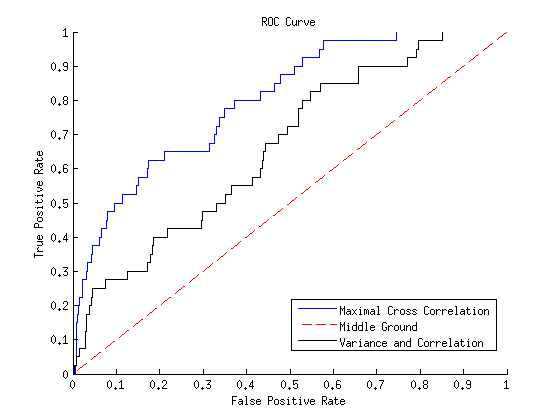
\includegraphics[width=0.48\textwidth]{MixedROC}
  \caption{A graph of the ROC curves for correlation and variance compared against that of maximal cross correlation} \label{fig:mixedROC}
\end{figure}

When looking at the resulting $STL_{max}$ graphs for an interictal and preictal segment, in Figure \ref{fig:STLMax}, there is an immediate disparity between the two.  This suggests that there may be some value to this feature that will confer some ability to distinguish the two classes. However, neither of the graphs seems to really resemble the pattern shown in Figure \ref{fig:origSTLMax} from the work of \cite{iasemidis05}.  The values during the preictal segment are not strictly lower than those during the interictal segment.  Furthermore, the values of the preictal segment do not approximate a strictly decreasing function, in fact quite the opposite.  One hypothesis to explain part of this difference is that the interictal and preictal segments in our work are not taken from closely spaced time points.  In fact, they must be at a minimum a week apart and are likely even much farther apart compared to \cite{iasemidis05} where they seizure events are only about 150 minutes apart.  The non-stationarity of EEG over time could be responsible for some of this difference. 

Despite the differences in appearance of $STL_{max}$, our algorithm accuracy improved to 72\% aucROC on Kaggle when incorporating the additional features.  Due to time constraints, and cluster allocation limits being reach, no graphics are currently available for the $STL_{max}$ algorithm.

\begin{figure}[!t]
\centering
  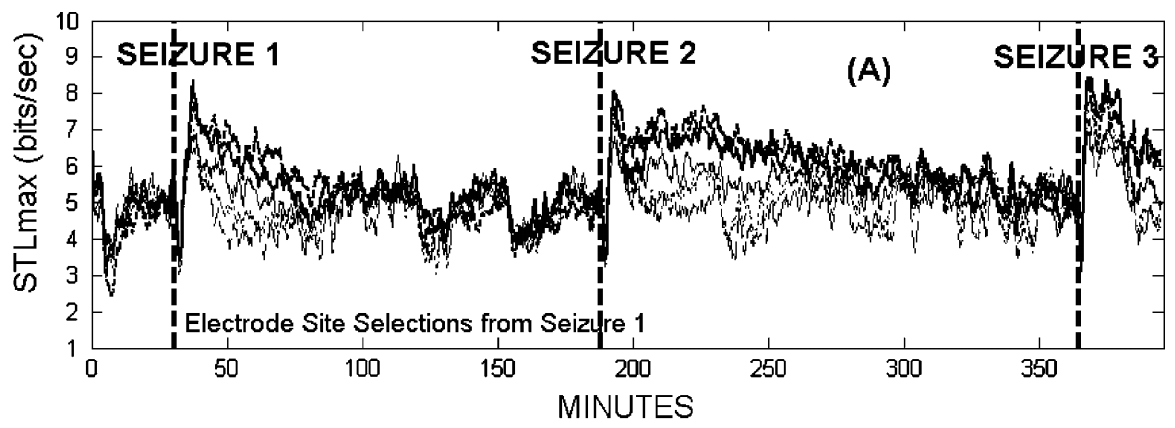
\includegraphics[width=0.48\textwidth]{origSTLMax}
  \caption{Plot of the $STL_{max}$ values as calculated by \cite{iasemidis05} for a series of three seizures} \label{fig:origSTLMax}
\end{figure}

\begin{figure}[!t]
  \centering{
    \subfloat[Interictal]{
      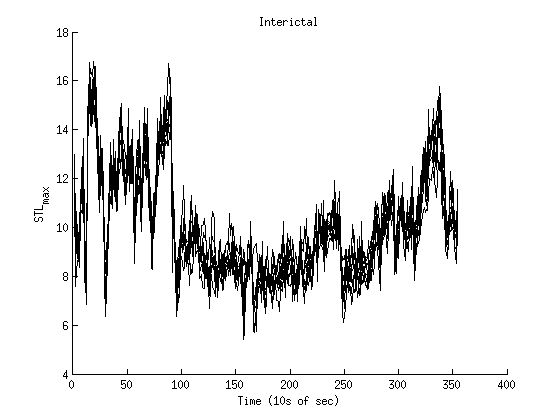
\includegraphics[width=0.3\textwidth]{interictal}%
      \label{fig:interictal}}
    \hfil
    \subfloat[Preictal]{
      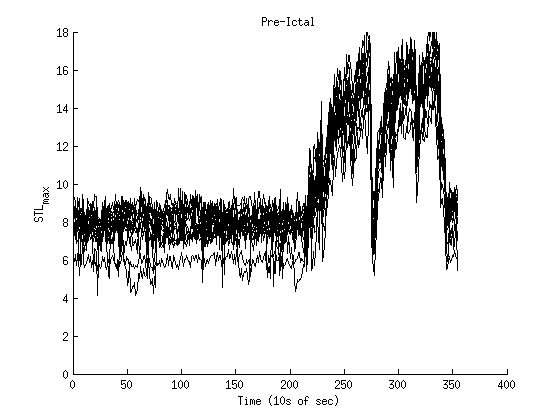
\includegraphics[width=0.3\textwidth]{preictal}%
      \label{fig:preictal}}
  }
  \caption{STLmax For two different 1hr segments of EEG} \label{fig:STLMax}
\end{figure}


%\section{Discussion} \label{sec:discussion}
%\input{Content/discussion}

\section{Conclusions and Future Work} \label{sec:conclusion}
One of the biggest limitations to the accuracy of our model was the limited amount of available preictal data.  There were twenty times more interictal training segments than their were preictal segments, and there were only about 24 preictal segments per subject.  This limited amount of data increases the likelihood that our SVM model will treat the preictal segments as noise and that greatly impacts our prediction accuracy.  Another substantial limitation was that imposed by available compute power.  The dataset for the Kaggle challenge was around 60 GB worth of data. Computation of the $STL_{max}$ algorithm on the full dataset took about ten days of compute time on an octacore compute node with 20GB of available RAM.  Having such long delays before knowing the results of the slightest change is quite preventative of fast progress.

Overall, I was able to achieve an aucROC score of 72\% in the Kaggle competition.  The competition came to a close on November 17th and the winner of the competition achieved an aucROC score of 84\%.  While these scores certainly indicate performance greater than random guessing, there is still a great deal of improvement that can be had.  One of the greatest difficulties in accurately predicting seizures is the lack of obvious feature choices.  To date, there has not been a particular feature that has been found to be a majority principal component of the prediction accuracy.  In future work I am interested in pursuing the effectiveness of convolutional network models and other unsupervised learning techniques.  Unsupervised learning techniques may hold the key to discovering relationships within the EEG that cannot be simply formulated with our knowledge today.






% if have a single appendix:
%\appendix[Proof of the Zonklar Equations]
% or
%\appendix  % for no appendix heading
% do not use \section anymore after \appendix, only \section*
% is possibly needed

% use appendices with more than one appendix
% then use \section to start each appendix
% you must declare a \section before using any
% \subsection or using \label (\appendices by itself
% starts a section numbered zero.)
%


%\appendices
%\section{Proof of the First Zonklar Equation}
%Appendix one text goes here.


% use section* for acknowledgement
\section*{Acknowledgments}
The authors would like to thank Dr. Ali Shoeb and Professor Zeeshan Syed for their help in directing the focus of our work and their invaluable adivising.


% Can use something like this to put references on a page
% by themselves when using endfloat and the captionsoff option.
\ifCLASSOPTIONcaptionsoff
  \newpage
\fi



% trigger a \newpage just before the given reference
% number - used to balance the columns on the last page
% adjust value as needed - may need to be readjusted if
% the document is modified later
%\IEEEtriggeratref{8}
% The "triggered" command can be changed if desired:
%\IEEEtriggercmd{\enlargethispage{-5in}}

% references section

% can use a bibliography generated by BibTeX as a .bbl file
% BibTeX documentation can be easily obtained at:
% http://www.ctan.org/tex-archive/biblio/bibtex/contrib/doc/
% The IEEEtran BibTeX style support page is at:
% http://www.michaelshell.org/tex/ieeetran/bibtex/
\bibliographystyle{IEEEtran}
% argument is your BibTeX string definitions and bibliography database(s)
\bibliography{IEEEabrv,BibTex/finalRefs}
\nocite{*}
%
% <OR> manually copy in the resultant .bbl file
% set second argument of \begin to the number of references
% (used to reserve space for the reference number labels box)
%\begin{thebibliography}{1}

%\bibitem{IEEEhowto:kopka}
%H.~Kopka and P.~W. Daly, \emph{A Guide to \LaTeX}, 3rd~ed.\hskip 1em plus
 % 0.5em minus 0.4em\relax Harlow, England: Addison-Wesley, 1999.

%\end{thebibliography}


% biography section
% 
% If you have an EPS/PDF photo (graphicx package needed) extra braces are
% needed around the contents of the optional argument to biography to prevent
% the LaTeX parser from getting confused when it sees the complicated
% \includegraphics command within an optional argument. (You could create
% your own custom macro containing the \includegraphics command to make things
% simpler here.)
\begin{biography}[{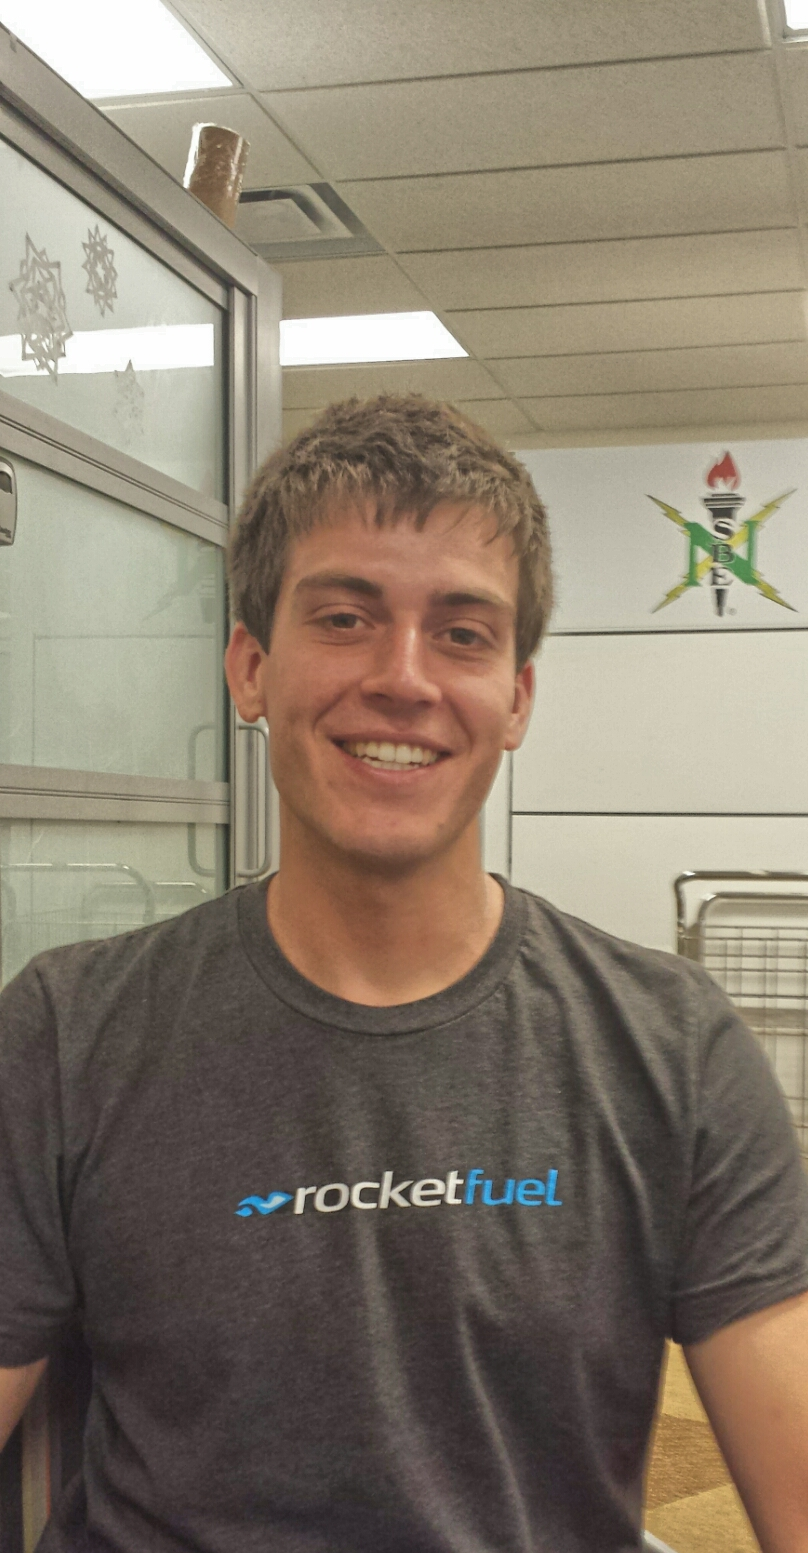
\includegraphics[width=1in,height=1.25in,clip,keepaspectratio]{chris}}]{Christopher Lesch}
graduated with a bachelors in Computer Engineering from the University of Michigan, Ann Arbor in 2012.  He is currently pursuing a masters degree from the University of Michigan, Ann Arbor in robotics and machine learning.  His primary focus is on machine learning and its applications to real time operating systems.
\end{biography}

% or if you just want to reserve a space for a photo:
%\begin{IEEEbiography}{Christopher Lesch}
% if you will not have a photo at all:
%\begin{IEEEbiographynophoto}{John Doe}
%Biography text here.
%\end{IEEEbiographynophoto}

% insert where needed to balance the two columns on the last page with
% biographies
%\newpage

%\begin{IEEEbiographynophoto}{Jane Doe}
%Biography text here.
%\end{IEEEbiographynophoto}

% You can push biographies down or up by placing
% a \vfill before or after them. The appropriate
% use of \vfill depends on what kind of text is
% on the last page and whether or not the columns
% are being equalized.

%\vfill

% Can be used to pull up biographies so that the bottom of the last one
% is flush with the other column.
%\enlargethispage{-5in}



% that's all folks
\end{document}


% An example of a floating figure using the graphicx package.
% Note that \label must occur AFTER (or within) \caption.
% For figures, \caption should occur after the \includegraphics.
% Note that IEEEtran v1.7 and later has special internal code that
% is designed to preserve the operation of \label within \caption
% even when the captionsoff option is in effect. However, because
% of issues like this, it may be the safest practice to put all your
% \label just after \caption rather than within \caption{}.
%
% Reminder: the "draftcls" or "draftclsnofoot", not "draft", class
% option should be used if it is desired that the figures are to be
% displayed while in draft mode.
%
%\begin{figure}[!t]
%\centering
%\includegraphics[width=2.5in]{myfigure}
% where an .eps filename suffix will be assumed under latex, 
% and a .pdf suffix will be assumed for pdflatex; or what has been declared
% via \DeclareGraphicsExtensions.
%\caption{Simulation Results}
%\label{fig_sim}
%\end{figure}

% Note that IEEE typically puts floats only at the top, even when this
% results in a large percentage of a column being occupied by floats.


% An example of a double column floating figure using two subfigures.
% (The subfig.sty package must be loaded for this to work.)
% The subfigure \label commands are set within each subfloat command, the
% \label for the overall figure must come after \caption.
% \hfil must be used as a separator to get equal spacing.
% The subfigure.sty package works much the same way, except \subfigure is
% used instead of \subfloat.
%
%\begin{figure*}[!t]
%\centerline{\subfloat[Case I]\includegraphics[width=2.5in]{subfigcase1}%
%\label{fig_first_case}}
%\hfil
%\subfloat[Case II]{\includegraphics[width=2.5in]{subfigcase2}%
%\label{fig_second_case}}}
%\caption{Simulation results}
%\label{fig_sim}
%\end{figure*}
%
% Note that often IEEE papers with subfigures do not employ subfigure
% captions (using the optional argument to \subfloat), but instead will
% reference/describe all of them (a), (b), etc., within the main caption.


% An example of a floating table. Note that, for IEEE style tables, the 
% \caption command should come BEFORE the table. Table text will default to
% \footnotesize as IEEE normally uses this smaller font for tables.
% The \label must come after \caption as always.
%
%\begin{table}[!t]
%% increase table row spacing, adjust to taste
%\renewcommand{\arraystretch}{1.3}
% if using array.sty, it might be a good idea to tweak the value of
% \extrarowheight as needed to properly center the text within the cells
%\caption{An Example of a Table}
%\label{table_example}
%\centering
%% Some packages, such as MDW tools, offer better commands for making tables
%% than the plain LaTeX2e tabular which is used here.
%\begin{tabular}{|c||c|}
%\hline
%One & Two\\
%\hline
%Three & Four\\
%\hline
%\end{tabular}
%\end{table}


% Note that IEEE does not put floats in the very first column - or typically
% anywhere on the first page for that matter. Also, in-text middle ("here")
% positioning is not used. Most IEEE journals use top floats exclusively.
% Note that, LaTeX2e, unlike IEEE journals, places footnotes above bottom
% floats. This can be corrected via the \fnbelowfloat command of the
% stfloats package.


